
We have also studied the solution NMR solved of a domain of adhesion exoprotein from Pediococcus pentosaceus. The
pdb id and CASP code of this 79 residue protein are 2KWY and T0569 respectively. We have compared the native structure with the
best model structure submitted for this target in CASP9. This model structute was submitted by the group " Mufold". ALl the
five model structures submitted by this group was found to be close. Thus we proceed by comparing only the native structure and 
the best predicted model of this target. Visualization upon superimposition of two structures reveals that 
the difference between the two structure is at the region consist of residues 48 to 65, where model1 is much more disordered compare to the 
native structure(see Figure~\ref{fig:fig:T0569}) . Other regions look similar for both the cases with of model1 is within 2.6 \AA 
rmsd value of the native structure. In this case we found that the confinement method predict that the predicted model is stable than the
native structure with a free energy difference of $9.4 \pm 0.7$ Kcal/Mol.   

\begin{figure}
\begin{center}
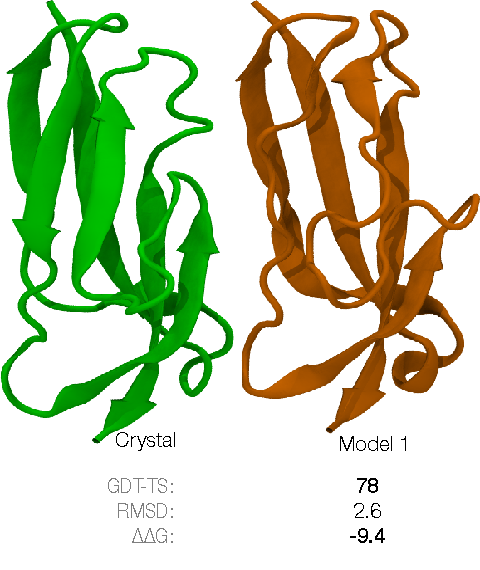
\includegraphics[width=3.2 in,height=3.8 in]{T0569.pdf}
\end{center}
\caption{Native and best model structure of a domain of adhesion exoprotein from Pediococcus pentosaceus (pdb id: 2KWY and CASP code: T0569). 
The best model was from the group "Mufold".}
\label{fig:T0569}
\end{figure}


\begin{table}
\label{table:casp_control}
\begin{center}
\begin{tabular}{l l l}\hline
    CASP Target  & PDB Identifier & $\Delta\Delta G_{native \to best decoy}$ (kcal/mol) \\ \hline
     T0531       &    2KJX        &          $12.49 \pm 0.70$ \\ \hline
     T0538       &    2L09        &          $-2.48 \pm 0.47$ \\ \hline
     T0540       &    3MX7        &          $22.00 \pm 0.49$ \\ \hline
     T0559       &    2L01        &          $2.24 \pm 0.24$ \\ \hline
     T0560       &    2L02        &          $22.15 \pm 0.49$ \\ \hline
     T0569       &    2KWY        &          $-9.40 \pm 0.69$  \\ \hline 
\end{tabular}
\end{center} 
